%! TEX root = ../main.tex
% ==============================================================
% IMMUTABLE — generated automatically, do not edit this block
%
% — Provenance ───────────────────────────────────────────────────
%   script            : analysis_scratch/reconstruction_A_vs_B.py
%   computed_in       : analysis_scratch/reconstruction_A_vs_B.py §5-§6 (PSD_wind = mean PSD residual_A(full) − mean PSD residual_A(no), per (freq,amp,mooring,panel) group)
%   plot_type         : reconstruction_pure_wind
%   data_class        : DELEG
%   generated_at      : 2026-05-02T16:55:47
%   findings_doc      : analysis_scratch/reconstruction_pure_wind_findings.md
%
% — Thesis context ──────────────────────────────────────────────
%   chapter           : 04
%   caption_label     : fig:ch04_reconstruction_pure_wind
%   caption_short     : 
%
% — Filters ────────────────────────────────────────────────────
%   panel             : full
%   wind              : no, full
%   amplitude [V]     : 
%   frequency [Hz]    : 1.3, 1.6
%   probes            : 
%   run_category      : 
%   quality_flag      : ok+probe_malfunction_secondary
%   mooring           : 
%
% — Data provenance ────────────────────────────────────────────
%   n_runs            : 103
%   in_probes_used    : 9373/170+9373/340
%   out_probes_used   : 12400/250
%   probe_configs     : march2026_better_rearranging
%   non_final_config_n: 
%   datasets        :
%     PROCESSED-20260326-ProbePos4_31_FPV_2-tett6roof-under9Mooring-height100-lowrange
%     PROCESSED-20260327-ProbePos4_31_FPV_2-tett6roof-under9Mooring30-height100-lowrange
%   run_paths       :
%     (omitted — aggregate over > threshold runs, see datasets)
%
% — Method / numerical parameters ─────────────────────────────
%   grouper           : per (freq, amp, mooring, panel) group; demo = single group
%   collapse_panels   : False
%   fft_window_hz     : 0.1
%   extra_params      : demo_run=1.4 Hz, 0.2 V, full panel; wind_band_hz=2.0-6.0; probes=['9373/170', '12400/250']; welch nperseg=min(len(residual), 4096), common grid 0-12.5 Hz @ 0.05 Hz
%
% — Summary stats cited in caption ────────────────────────────
%   stat:n_groups     : 13
%   stat:stokes_frac_in_median_pct : 18.4
%   stat:stokes_frac_in_max_pct : 58.2
%   stat:stokes_frac_out_median_pct : 17.3
%
% — Subfigures available ───────────────────────────────────────
%     FIGURES/ch04_reconstruction_pure_wind.pdf
% ── end immutable block ─────────────────────────────────────────
\begin{figure}[htbp]
  \centering
  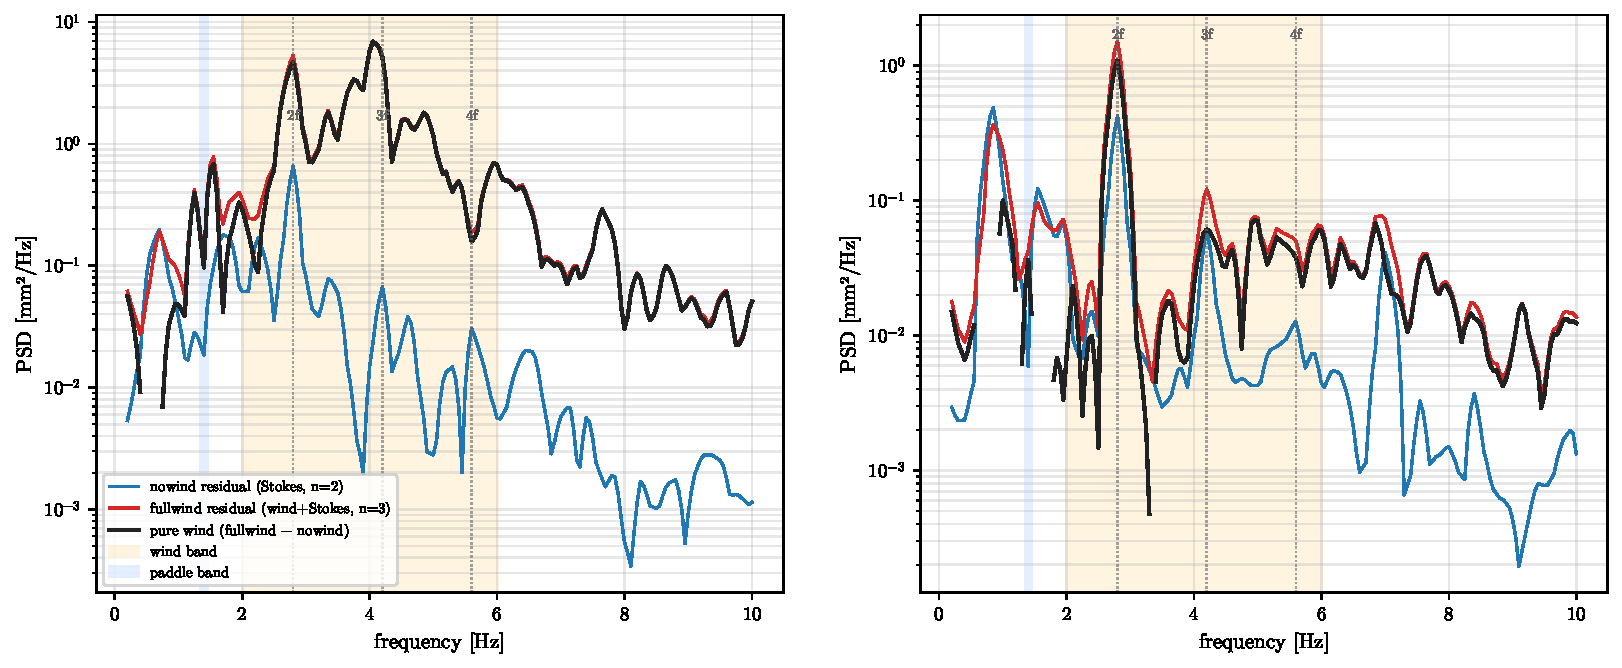
\includegraphics[width=\linewidth]{FIGURES/ch04_reconstruction_pure_wind.pdf}
  \caption{
    Mean residual power spectra at the IN probe (left, 9373/170) and OUT probe (right, 12400/250) for the 1.4\,Hz / 0.20\,V / full-panel group. No-wind residuals (blue) carry only paddle-linked Stokes harmonics; full-wind residuals (red) carry Stokes plus wind-wave energy. Subtracting the no-wind baseline from the full-wind residual (black) isolates pure wind. Vertical dotted lines mark $2f$, $3f$ and $4f$, all of which fall inside the wind band (2--6\,Hz, orange) at thesis paddle frequencies. Across the full thesis scope ($n=13$ frequency--amplitude groups with matched no-wind/full-wind coverage), the Stokes-subtraction correction removes a median $18$\,\% of the naive ``wind'' energy at IN and $17$\,\% at OUT (up to $58$\,\% at the IN / 0.3\,V high-frequency corner). Any wind-energy metric that integrates a wave run's residual over 2--6\,Hz without this subtraction mis-attributes paddle Stokes harmonics as wind.
  }
  \label{fig:ch04_reconstruction_pure_wind}
\end{figure}
